% main.tex - 主文件
\documentclass[a4paper,12pt]{article}
\PassOptionsToPackage{quiet}{fontspec}
\usepackage[UTF8,heading = true]{ctex}  % 中文支持
\usepackage{geometry}  % 页面设置
\usepackage{graphicx}  % 图片支持
\usepackage{subfigure} % 用于子图排列
\usepackage{amsmath}  % 数学公式
\usepackage{booktabs}  % 表格
\usepackage{fontspec}  % 字体设置
\setmainfont{Times New Roman}  % 设置英文默认字体为Times New Roman
\usepackage{caption}  % 图表标题
\usepackage{fancyhdr}  % 页眉页脚
\usepackage{enumitem}  % 列表环境
\usepackage{hyperref}  % 超链接
\usepackage[sort&compress]{natbib}  % 用于管理参考文献格式
\usepackage{lmodern}

% 页面设置
\geometry{top=2.5cm,bottom=2.5cm,left=3cm,right=2.5cm}

% 页眉页脚设置
\pagestyle{fancy}
\fancyhf{}
\renewcommand{\headrulewidth}{0pt}
\fancyfoot[C]{-~\thepage~-}

% 标题格式设置
% format.tex - 格式设置文件
\newcommand{\chineseabstract}{
    \noindent\zihao{-5}\songti\textbf{摘要:}\songti
}

\newcommand{\chinesekeywords}{
    \noindent\zihao{-5}\songti\textbf{关键词:}
}

\newcommand{\englishabstract}{
    \noindent\zihao{5}{\bfseries\fontspec{Times New Roman}[Weight=Bold]Abstract: }
}

\newcommand{\englishkeywords}{
    \noindent\zihao{5}{\bfseries\fontspec{Times New Roman}[Weight=Bold]Key words: }
}

% 节标题格式
\ctexset{section={format={\zihao{4}\heiti}}}
\ctexset{subsection={format={\zihao{5}\heiti}}}
\ctexset{subsubsection={format={\zihao{5}\songti}}}

% 图表标题格式
\DeclareCaptionFont{sfive}{\zihao{-5}}
\captionsetup[figure]{font=sfive,justification=centering}
\captionsetup[table]{font=sfive,justification=centering}

% 修改后的方案
\newcommand{\bottomnote}{
    \vfill
    \bottomnotefont
    \bottomnotespacing
    \noindent\rule{\linewidth}{0.4pt}\\
    \noindent 收稿日期:20**-**-**\\
    \noindent 基金项目:基金名称(编号)(六号字体):国家自然科学基金资助项目(00000001);\\
    \noindent 通信作者:李~三(1998——),男,教授,博士生导师,博士,研究方向为图像处理、数据挖掘等. E-mail: ****@shu.edu.cn (建议使用单位邮箱)
}  % 导入格式设置文件

% 文档信息
\title{\heiti\zihao{2} 论文标题论文标题}
\author{}
\date{\vspace{-3em}}

\begin{document}

% 标题页
% title.tex - 标题页
\maketitle
% 作者信息
{\centering\kaishu\zihao{4}
    张一一\textsuperscript{1},李~三\textsuperscript{2},王~五\textsuperscript{1}\\[2ex]
    
    \zihao{-5}
    (1. ***大学 **************学院,上海 2004**;\\
    2. ***大学 **************学院,江苏 苏州 2151**;)\\[2ex]
}

% 中文摘要
\chineseabstract
中文摘要内容...

\chinesekeywords
关键词一;关键词二;关键词三

% 中图分类号
\noindent\zihao{-5}\songti
\textbf{中图分类号:} \quad \textbf{文献标志码:}A\newline

% 英文标题
{\centering
    \zihao{4}\textbf{English title english title english title}\\[2ex]
    
    \zihao{5}
    ZHANG Yiyi\textsuperscript{1}, LI San\textsuperscript{2}, WANG Wu\textsuperscript{1}\\[2ex]
    
    \zihao{-5}
    (1. School of *************, ********** University, Shanghai 2004**, China;\\
    2. School of *************, ********** University, Suzhou 2151**, Jiangsu, China;)\\[2ex]
}

% 英文摘要
\englishabstract
English abstract content...

\englishkeywords
key word one; key word two; key word three\\[4ex]  % 导入标题页

% 正文部分
% content.tex - 正文内容
\section{提出问题}
\subsection{提出问题一}
\subsubsection{三级标题}
正文内容...\cite{ref1}\cite{ref2}

% 图片示例
\begin{figure}[htbp]
    \centering
    \subfigure[图题]{
        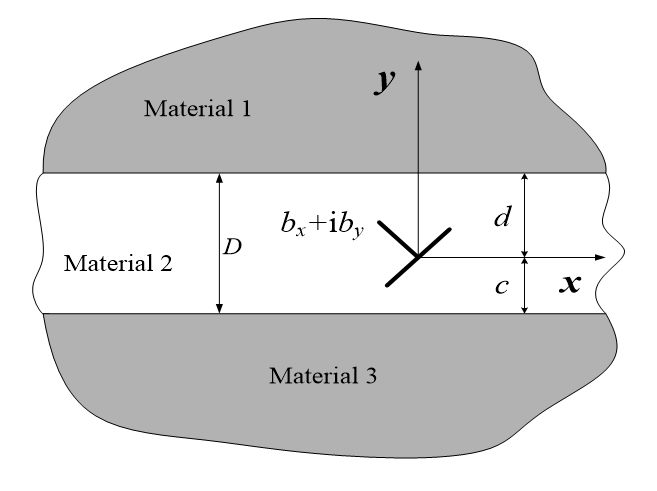
\includegraphics[width=0.45\textwidth]{figure/example.jpg}
    }
    \subfigure[图题]{
        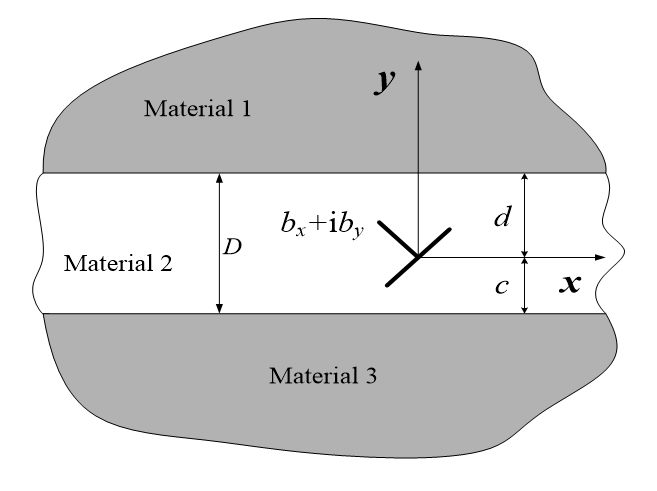
\includegraphics[width=0.45\textwidth]{figure/example.jpg}
    }
    \caption{位于三层材料体系中的位错示意图}
    \label{fig:dislocation}
\end{figure}

% 表格示例
\begin{table}[htbp]
    \centering
    \caption{表题}
    \label{tab:example}
    \begin{tabular}{ccc}
        \toprule
        速度/(m.s\textsuperscript{-1}) & 时间/s & 频率/kHz \\
        \midrule
        第一次 & ... & ... \\
        第二次 & ... & ... \\
        第三次 & ... & ... \\
        \bottomrule
    \end{tabular}
\end{table}

% 公式示例
\begin{equation}
    E = mc^2
    \label{eq:example}
\end{equation}

% ==================================  % 导入正文内容

% 致谢
% acknowledgment.tex - 致谢
\section*{\zihao{-5}\heiti 致谢}
\zihao{-5}\songti
感谢赵六六教授对本工作的大力支持,在此表示感谢!  % 导入致谢

% 参考文献
% references.tex - 参考文献
\bibliographystyle{plain}  % 可选择不同的引用样式,如plain、unsrt、alpha等
\zihao{-5}
\bibliography{ref}  % 不需要加.bib后缀  % 导入参考文献

\end{document}
